\documentclass[12pt,letterpaper]{article}
\usepackage[utf8]{inputenc}
\usepackage[spanish]{babel}
\usepackage{graphicx}
\usepackage[left=2cm,right=2cm,top=2cm,bottom=2cm]{geometry}
\usepackage{graphicx} % figuras
% \usepackage{subfigure} % subfiguras
\usepackage{float} % para usar [H]
\usepackage{amsmath}
%\usepackage{txfonts}
\usepackage{stackrel} 
\usepackage{graphicx}
\usepackage{subfig}
\usepackage{hyperref}
\usepackage{multirow}
\usepackage{enumerate} % enumerados
\renewcommand{\labelitemi}{$-$}
\renewcommand{\labelitemii}{$\cdot$}
% \author{}
% \title{Caratula}
\begin{document}

% Fancy Header and Footer
% \usepackage{fancyhdr}
% \pagestyle{fancy}
% \cfoot{}
% \rfoot{\thepage}
%

% \usepackage[hidelinks]{hyperref} % CREA HYPERVINCULOS EN INDICE
  
% \author{}
\title{Caratula}

\begin{titlepage}
    \begin{center}
    \begin{figure}[htb]
    \begin{center}
    
\includegraphics[width=3.5cm]{./img/upt.jpg}
    \end{center}
    \end{figure}
    
    \vspace*{0.15in}
    \begin{Large}
    \textbf{UNIVERSIDAD PRIVADA DE TACNA}\\
    \end{Large}
    
    \vspace*{0.1in}
    \begin{Large}
    \textbf{FACULTAD DE INGENIERIA} \\
    \end{Large}
    
    \vspace*{0.1in}
    \begin{Large}
    \textbf{ESCUELA PROFESIONAL DE INGENIERIA DE SISTEMAS} \\
    \end{Large}
    
    \vspace*{0.5in}
    \begin{Large}
    \textbf{TITULO:}\\
    \end{Large}
    

\vspace*{0.1in}
\begin{Large}
    PRACTICA DE LABORATORIO 05: ELABORACION DE REPORTES OPERACIONALES\\
\end{Large}

\vspace*{0.3in}
\begin{Large}
\textbf{Curso:} \\
\end{Large}

\vspace*{0.1in}
\begin{large}
    Inteligencia De Negocios\\
\end{large}

\vspace*{0.3in}
\begin{Large}
\textbf{Docente:} \\
\end{Large}

\vspace*{0.1in}
\begin{large}
Ing. Patrick Cuadros Quiroga\\
\end{large}

\vspace*{0.2in}
\vspace*{0.1in}
\begin{large}
\textbf{Alumno:} \\
\begin{flushleft}
 Herrera Amezquita, Derian Francisco		\hfill	(2017059489) \\


\end{flushleft}
\end{large}
\vspace*{0.1in}
\begin{large}
Tacna - Perú\\
\end{large}
\vspace*{0.1in}
\begin{large}
2021\\
\end{large}

\end{center}

\end{titlepage}



\tableofcontents % INDICE
\thispagestyle{empty} % INDICE SIN NUMERO
\newpage
\setcounter{page}{1} % REINICIAR CONTADOR DE PAGINAS DESPUES DEL INDICE


\section{Objetivos}
A
\section{Requerimientos}
Conocimientos
\\Para el desarrollo de esta práctica se requerirá de los siguientes conocimientos básicos:
\\- Conocimientos básicos de administración de base de datos Microsoft SQL Server.
\\- Conocimientos básicos de SQL.
\\\\Software
\\\\Asimismo se necesita los siguientes aplicativos:
\\\\- Microsoft SQL Server 2017 o superior

\section{Desarrollo}
Nombre de la base de datos: Control\_De\_Libros\_Sucarnet
\subsection{Parte I}
Debe crear la base de datos, tomando en cuenta las relaciones entre las
tablas (llaves primarias y llaves foráneas). Así como se presenta en la siguiente
figura:
\begin{center}
    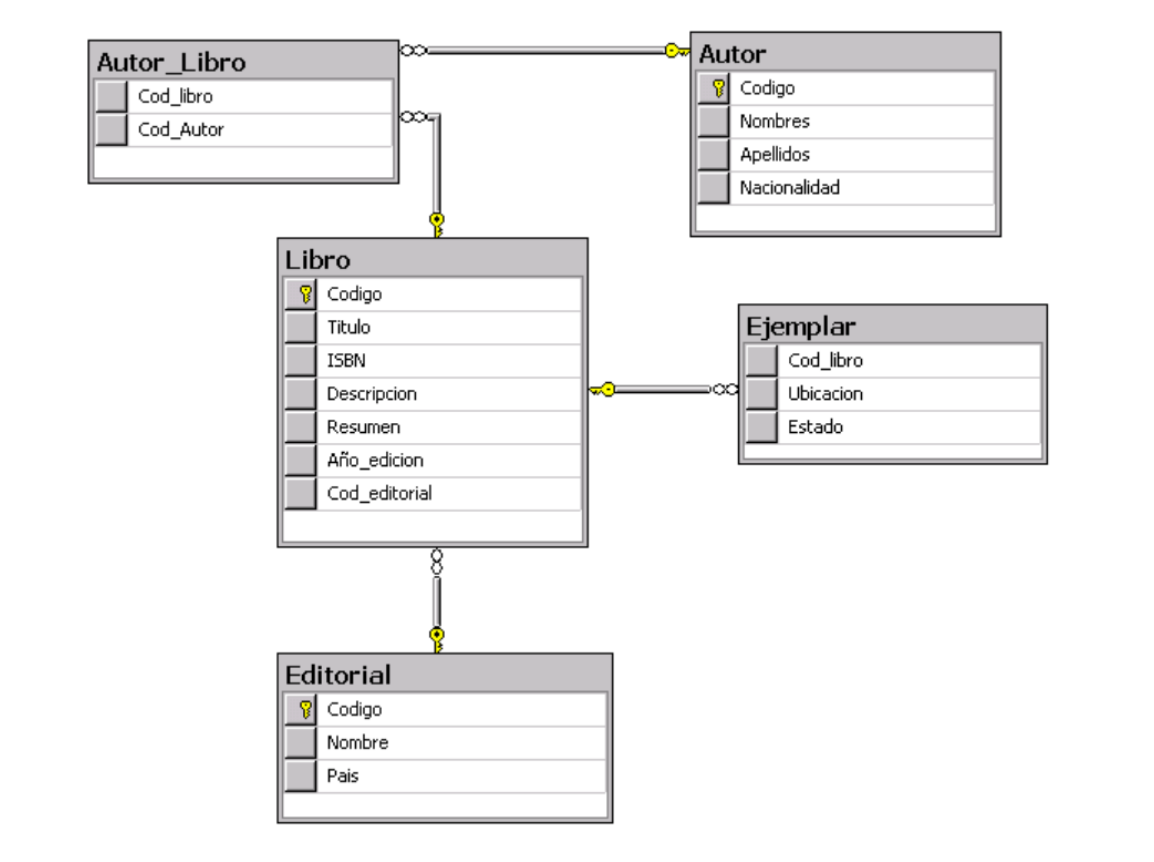
\includegraphics[width=14cm]{img/graph.png}  
\end{center}
\begin{center}
    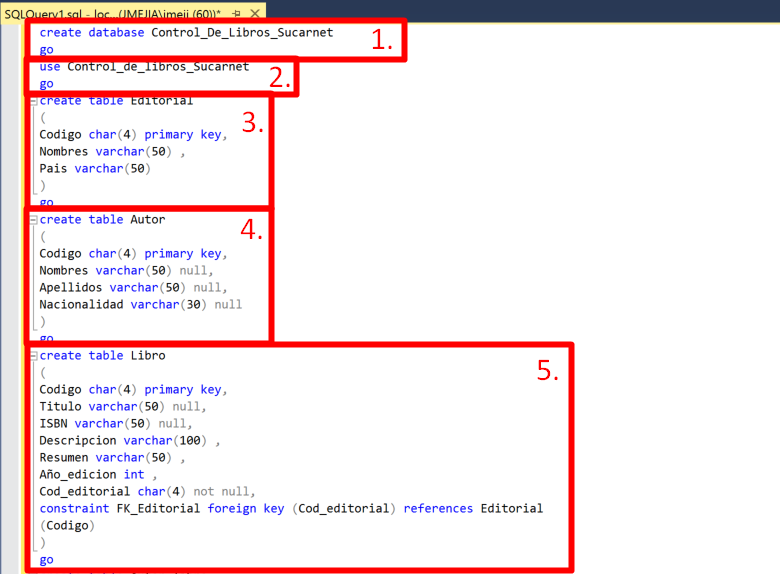
\includegraphics[width=17cm]{img/1.png}
    \vspace{2cm}  
\end{center}
\begin{center}
    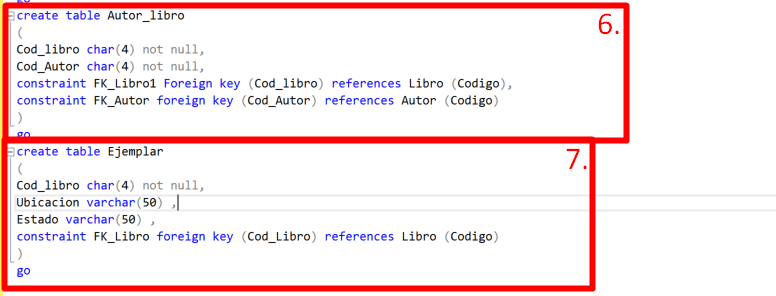
\includegraphics[width=17cm]{img/2.png}
    \vspace{3cm}  
\end{center}
Agregar los siguientes datos a cada tabla.
\begin{center}
    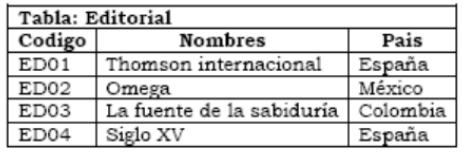
\includegraphics[width=10cm]{img/graph1.png}  
\end{center}
\begin{center}
    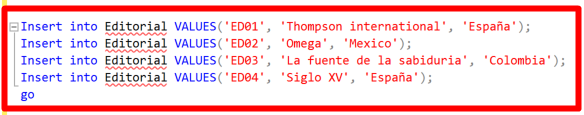
\includegraphics[width=15cm]{img/3.png}  
\end{center}
\begin{center}
    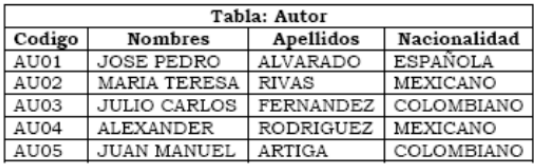
\includegraphics[width=12cm]{img/graph4.png}  
\end{center}
\begin{center}
    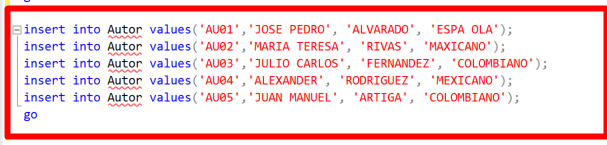
\includegraphics[width=13cm]{img/5.png}  
\end{center}
\begin{center}
    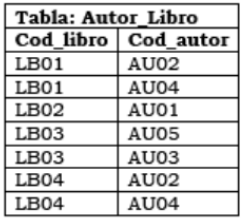
\includegraphics[width=5cm]{img/graph3.png}  
\end{center}
\begin{center}
    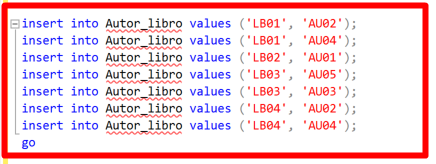
\includegraphics[width=11cm]{img/6.png}  
\end{center}
\begin{center}
    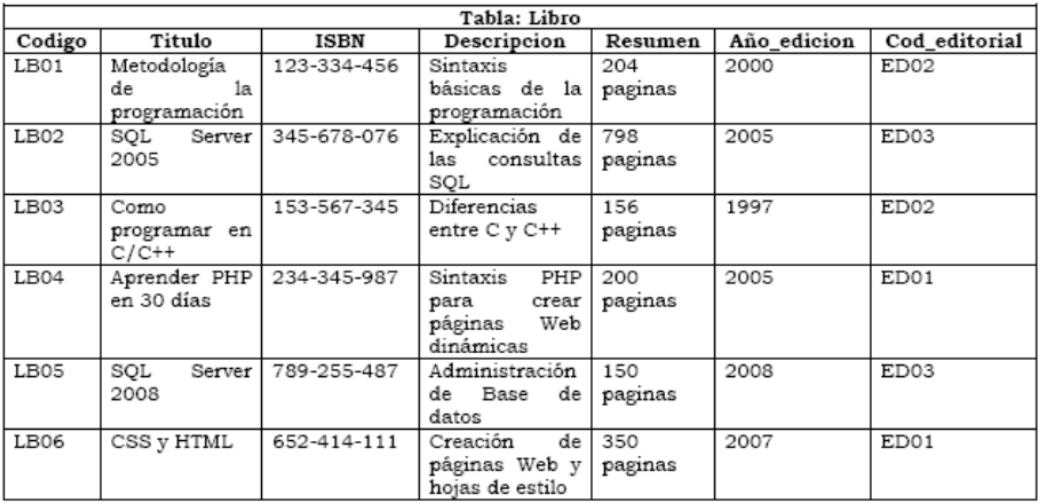
\includegraphics[width=14cm]{img/graph5.png}  
\end{center}
\begin{center}
    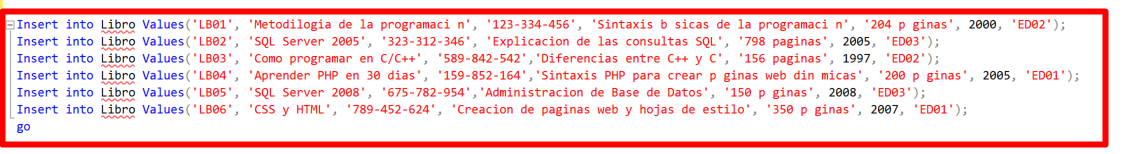
\includegraphics[width=18cm]{img/4.png}  
\end{center}
\begin{center}
    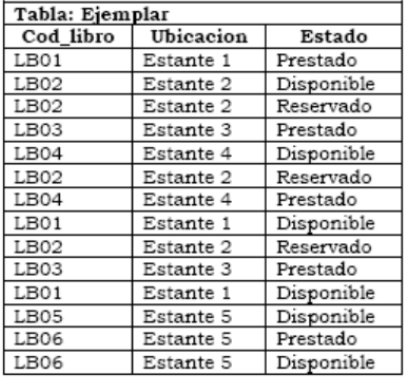
\includegraphics[width=7cm]{img/graph2.png}  
\end{center}
\begin{center}
    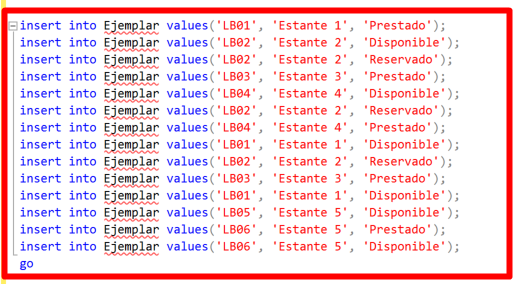
\includegraphics[width=11cm]{img/7.png}  
\end{center}

\subsection{Parte II}
Crear las siguientes consultas SQL:
\\Utilizando consultas a múltiples tablas resolver los siguientes problemas:
\\\\a. Se desea mostrar los datos de los autores junto con los títulos de libros que han escrito.
Ordenarlos en forma descendente por el nombre del autor.
\begin{center}
    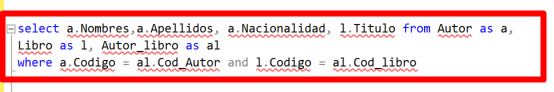
\includegraphics[width=14cm]{img/8.png}  
\end{center}
\begin{center}
    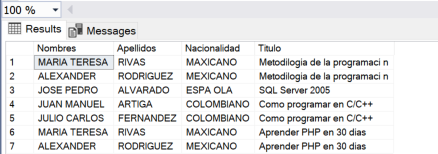
\includegraphics[width=11cm]{img/9.png}  
\end{center}
b. Se desea conocer todos los autores que tienen libros que han sido publicados por la
editorial “Omega”.
\begin{center}
    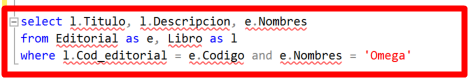
\includegraphics[width=12cm]{img/10.png}  
\end{center}
\begin{center}
    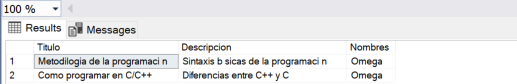
\includegraphics[width=12cm]{img/11.png}  
\end{center}
c. Mostrar cuántos ejemplares hay por cada libro. Titulo, ejemplar
\begin{center}
    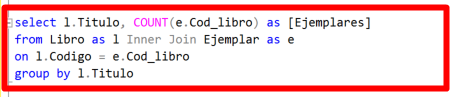
\includegraphics[width=11cm]{img/12.png}  
\end{center}
\begin{center}
    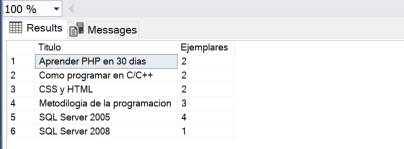
\includegraphics[width=12cm]{img/13.png}  
\end{center}
d. Mostrar los títulos de los libros donde el estado sea “Prestado”.
\begin{center}
    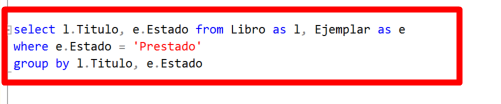
\includegraphics[width=12cm]{img/14.png}  
\end{center}
\begin{center}
    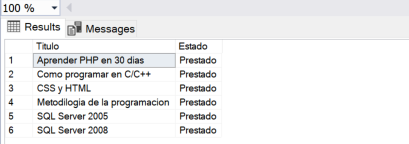
\includegraphics[width=11cm]{img/15.png}
    \vspace{1cm}    
\end{center}
e. Se desea mostrar los libros que se han editados entre el 2000 y 2007. Ordenarlos en
forma ascendente.
\begin{center}
    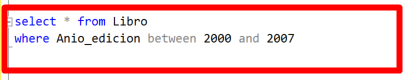
\includegraphics[width=11cm]{img/16.png}  
\end{center}
\begin{center}
    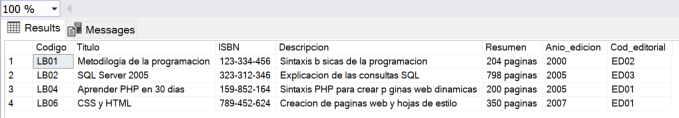
\includegraphics[width=15cm]{img/17.png}
    \vspace{1cm}  
\end{center}
f. Mostrar cuántos libros que se han prestado y agruparlos por el estante
\begin{center}
    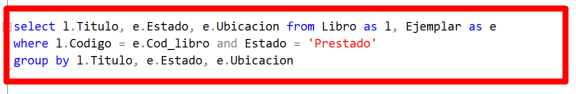
\includegraphics[width=12cm]{img/18.png}  
\end{center}
\begin{center}
    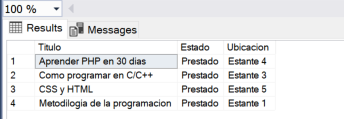
\includegraphics[width=10cm]{img/19.png}  
\end{center}

\subsection{Parte III}
Generar reportes operacionales de la parte II utilizando un visualizador Power BI, Tableau o
Qlik Sense
\begin{center}
    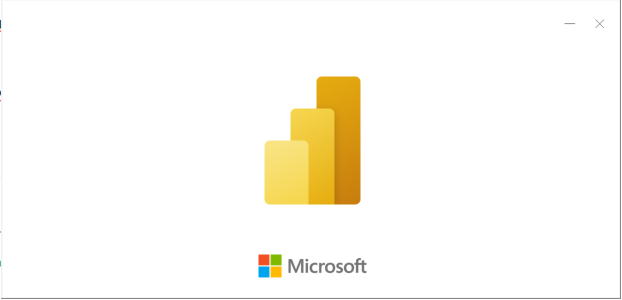
\includegraphics[width=8cm]{img/power.png}  
\end{center}
a. Se desea mostrar los datos de los autores junto con los títulos de libros que han escrito.
Ordenarlos en forma descendente por el nombre del autor.
\begin{center}
    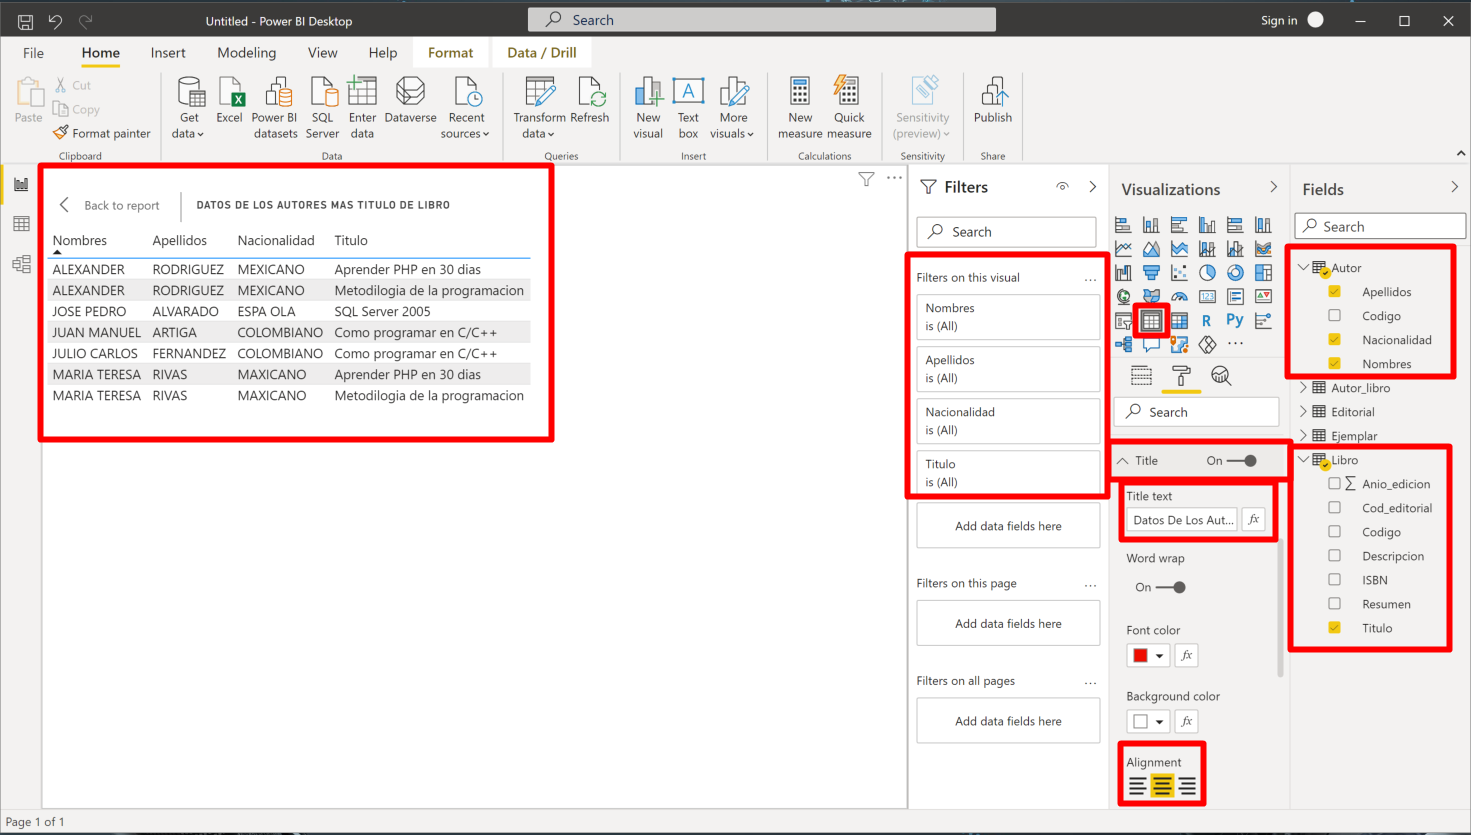
\includegraphics[width=13cm]{img/26.png}  
\end{center}
b. Se desea conocer todos los autores que tienen libros que han sido publicados por la
editorial “Omega”.
\begin{center}
    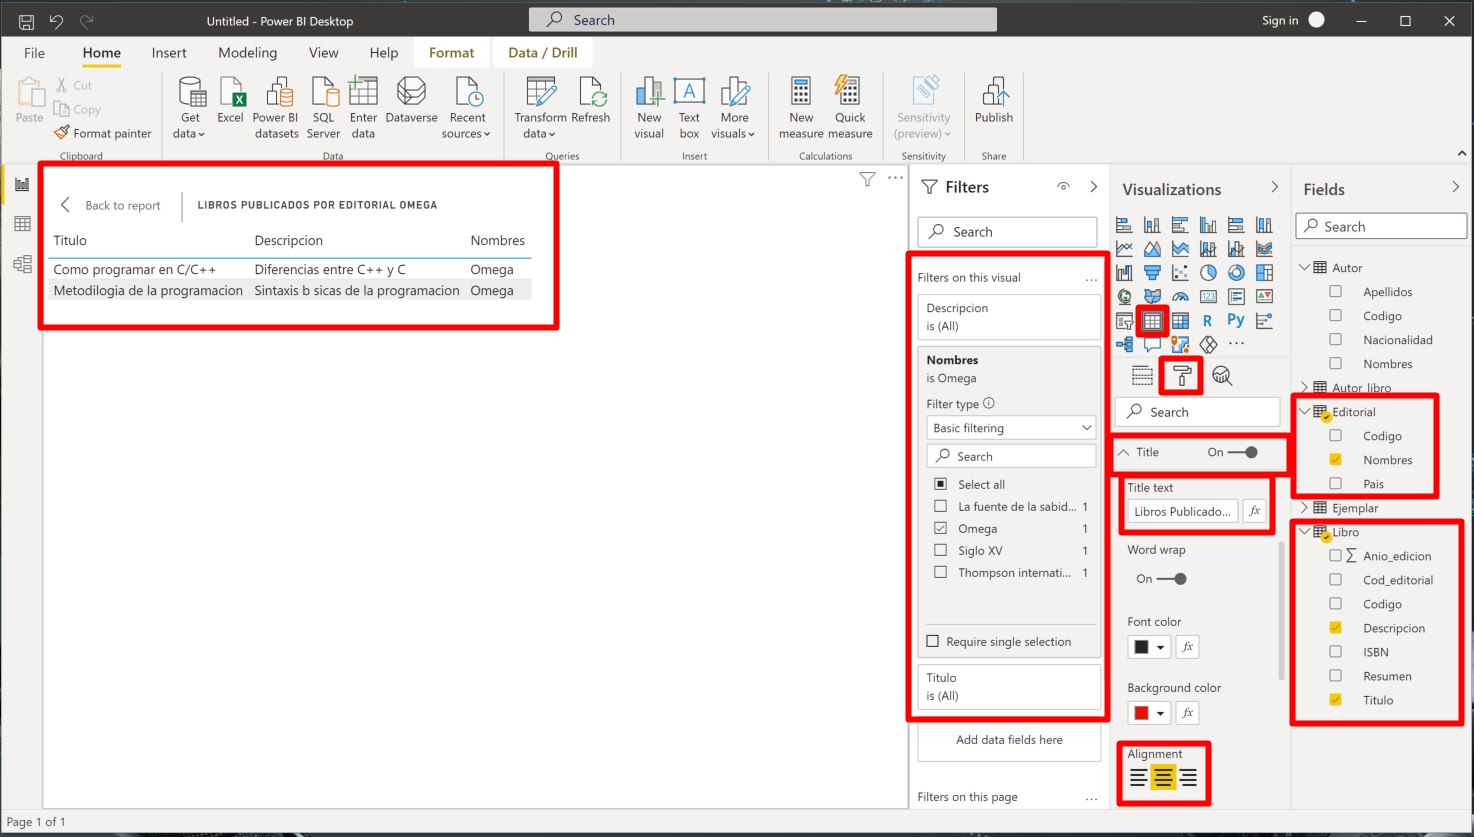
\includegraphics[width=13cm]{img/27.png}  
\end{center}
c. Mostrar cuántos ejemplares hay por cada libro. Titulo, ejemplar
\begin{center}
    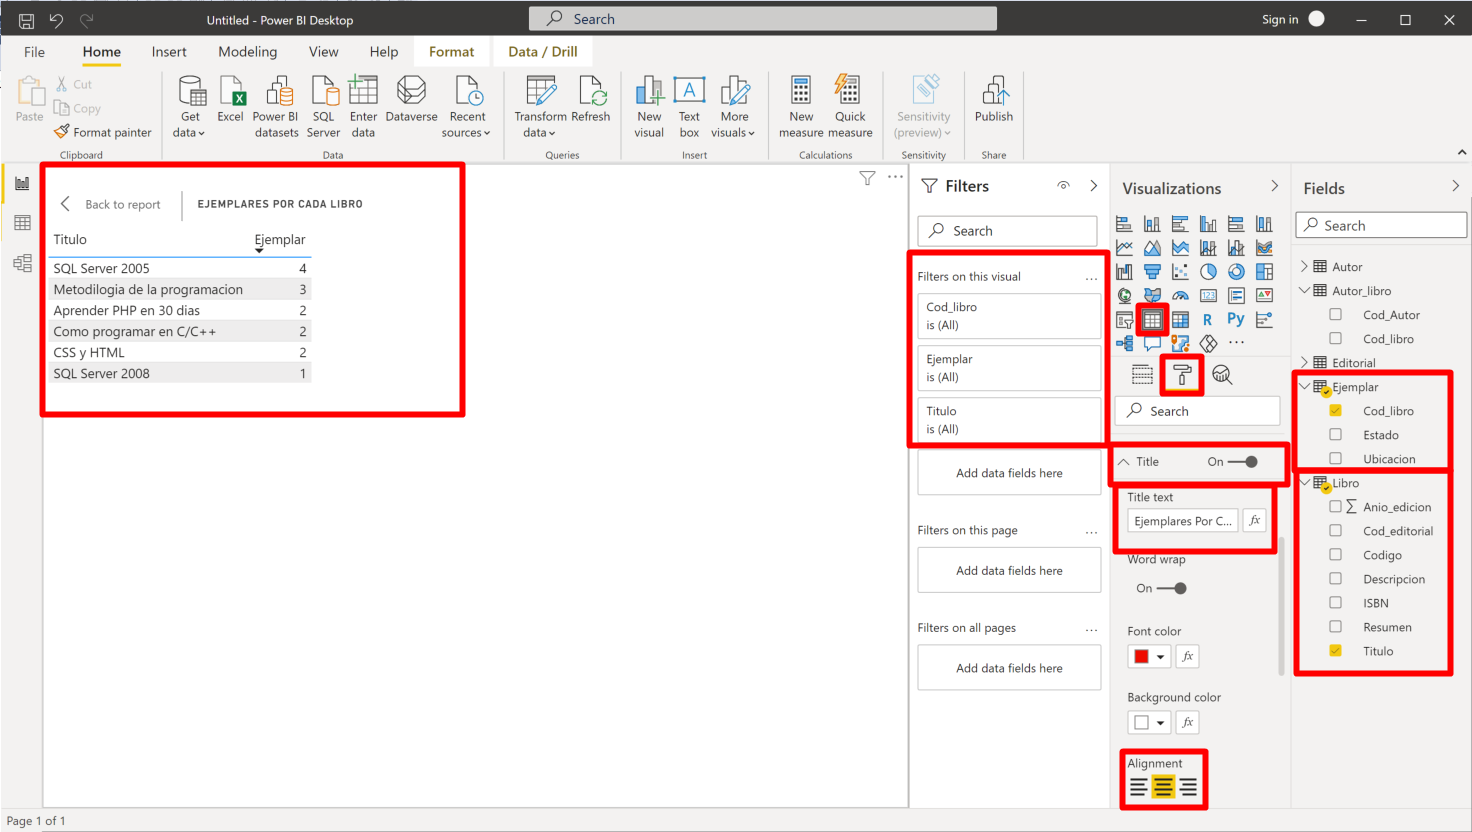
\includegraphics[width=16cm]{img/28.png}  
    \vspace{1cm}
\end{center}
d. Mostrar los títulos de los libros donde el estado sea “Prestado”.
\begin{center}
    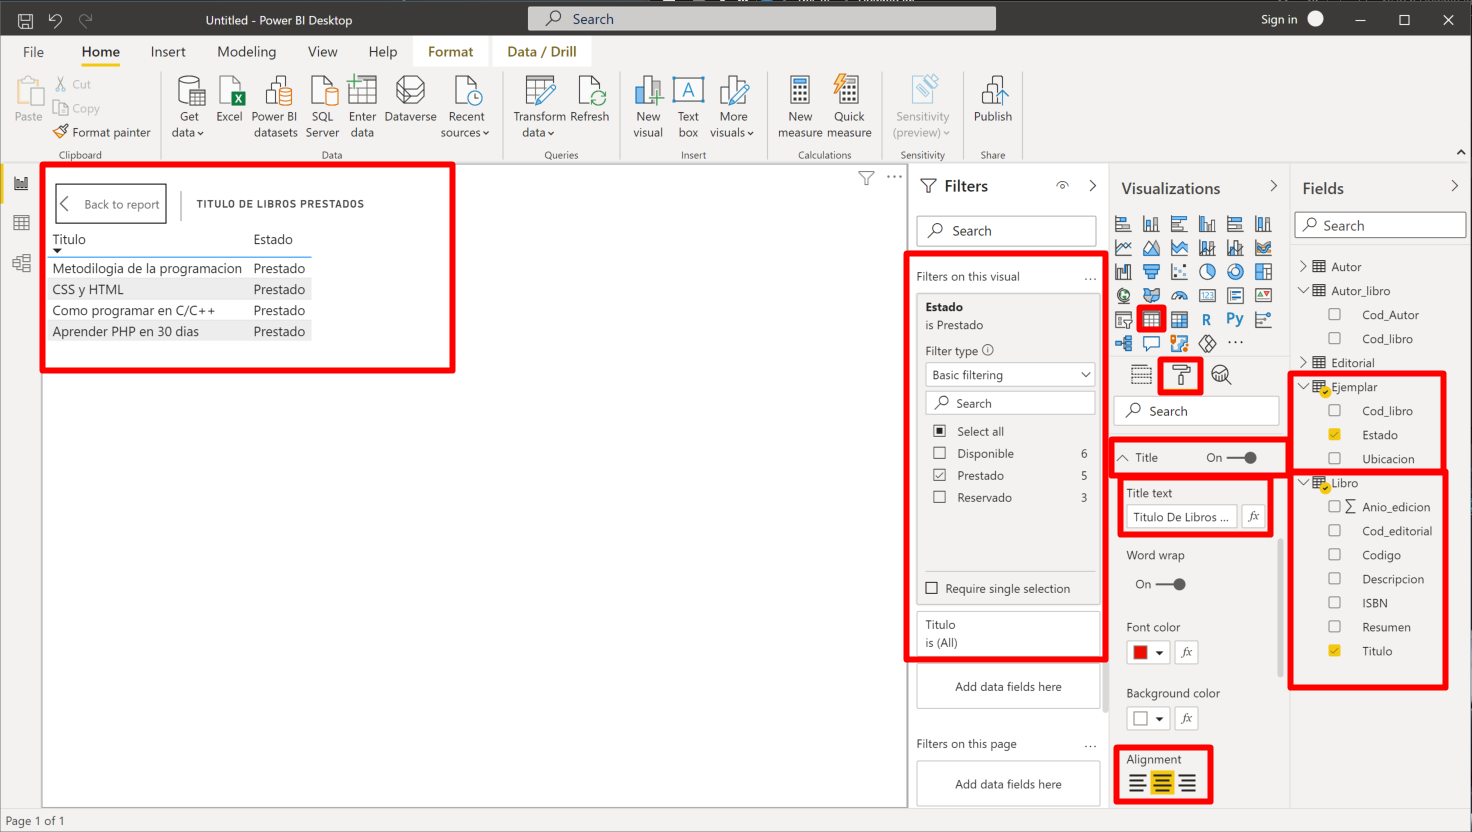
\includegraphics[width=16cm]{img/30.png}
    \vspace{3cm}  
\end{center}
e. Se desea mostrar los libros que se han editados entre el 2000 y 2007. Ordenarlos en
forma ascendente.
\begin{center}
    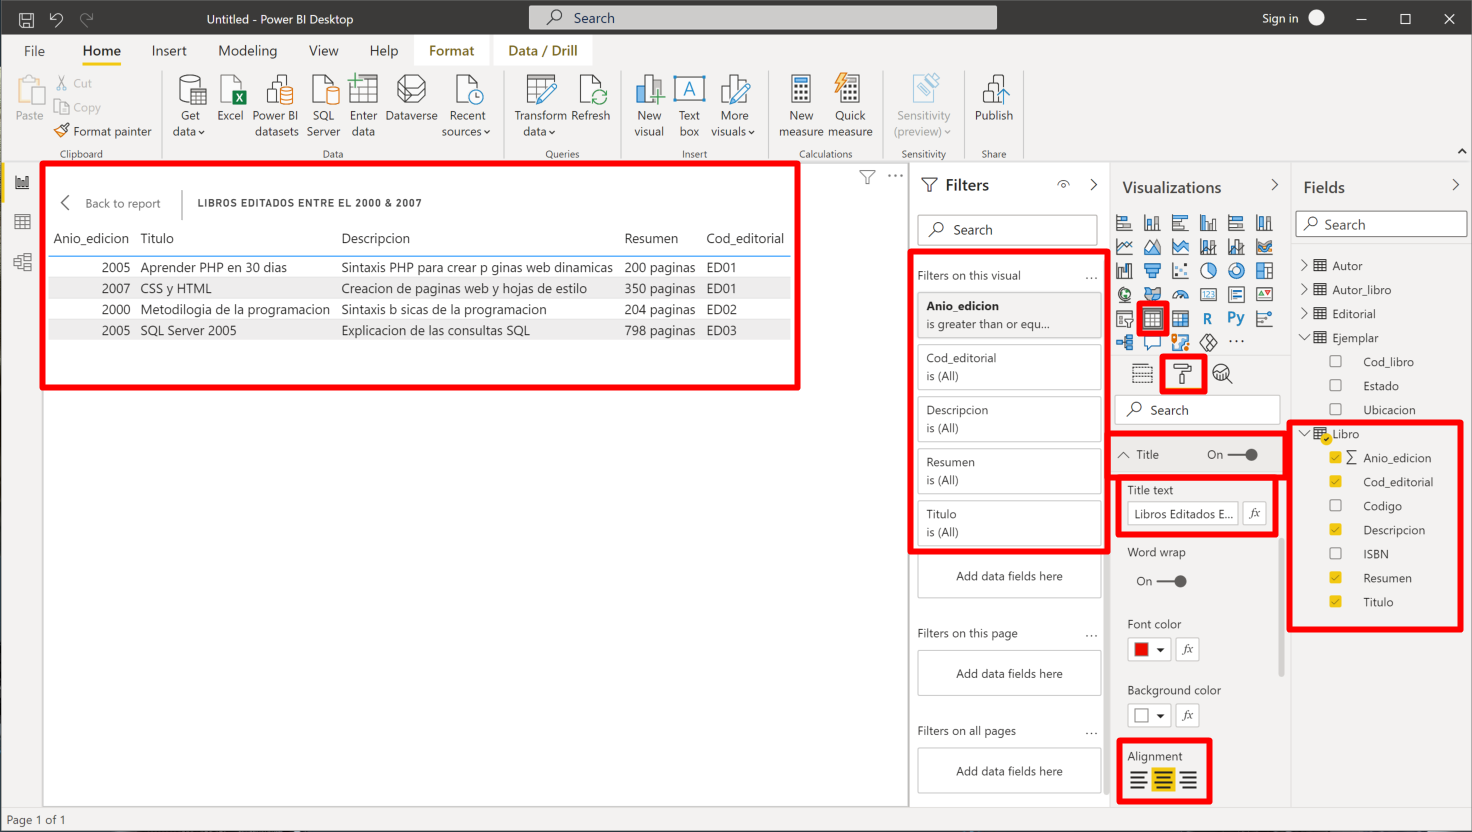
\includegraphics[width=16cm]{img/25.png}
    \vspace{1cm}  
\end{center}
f. Mostrar cuántos libros que se han prestado y agruparlos por el estante
\begin{center}
    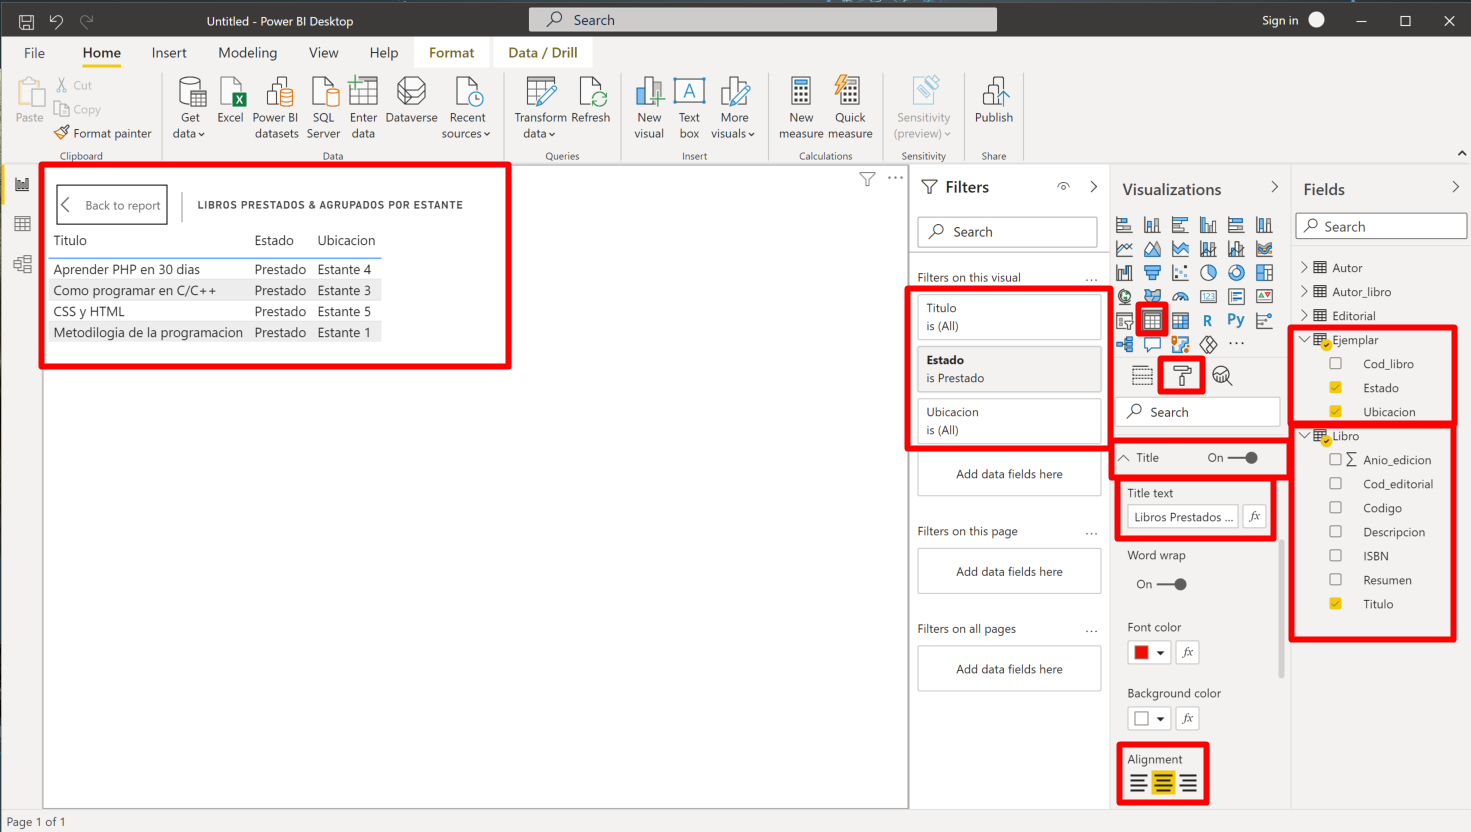
\includegraphics[width=16cm]{img/29.png} 
    \vspace{2cm} 
\end{center}
Resultado Final De Los Reportes en Power BI:
\begin{center}
    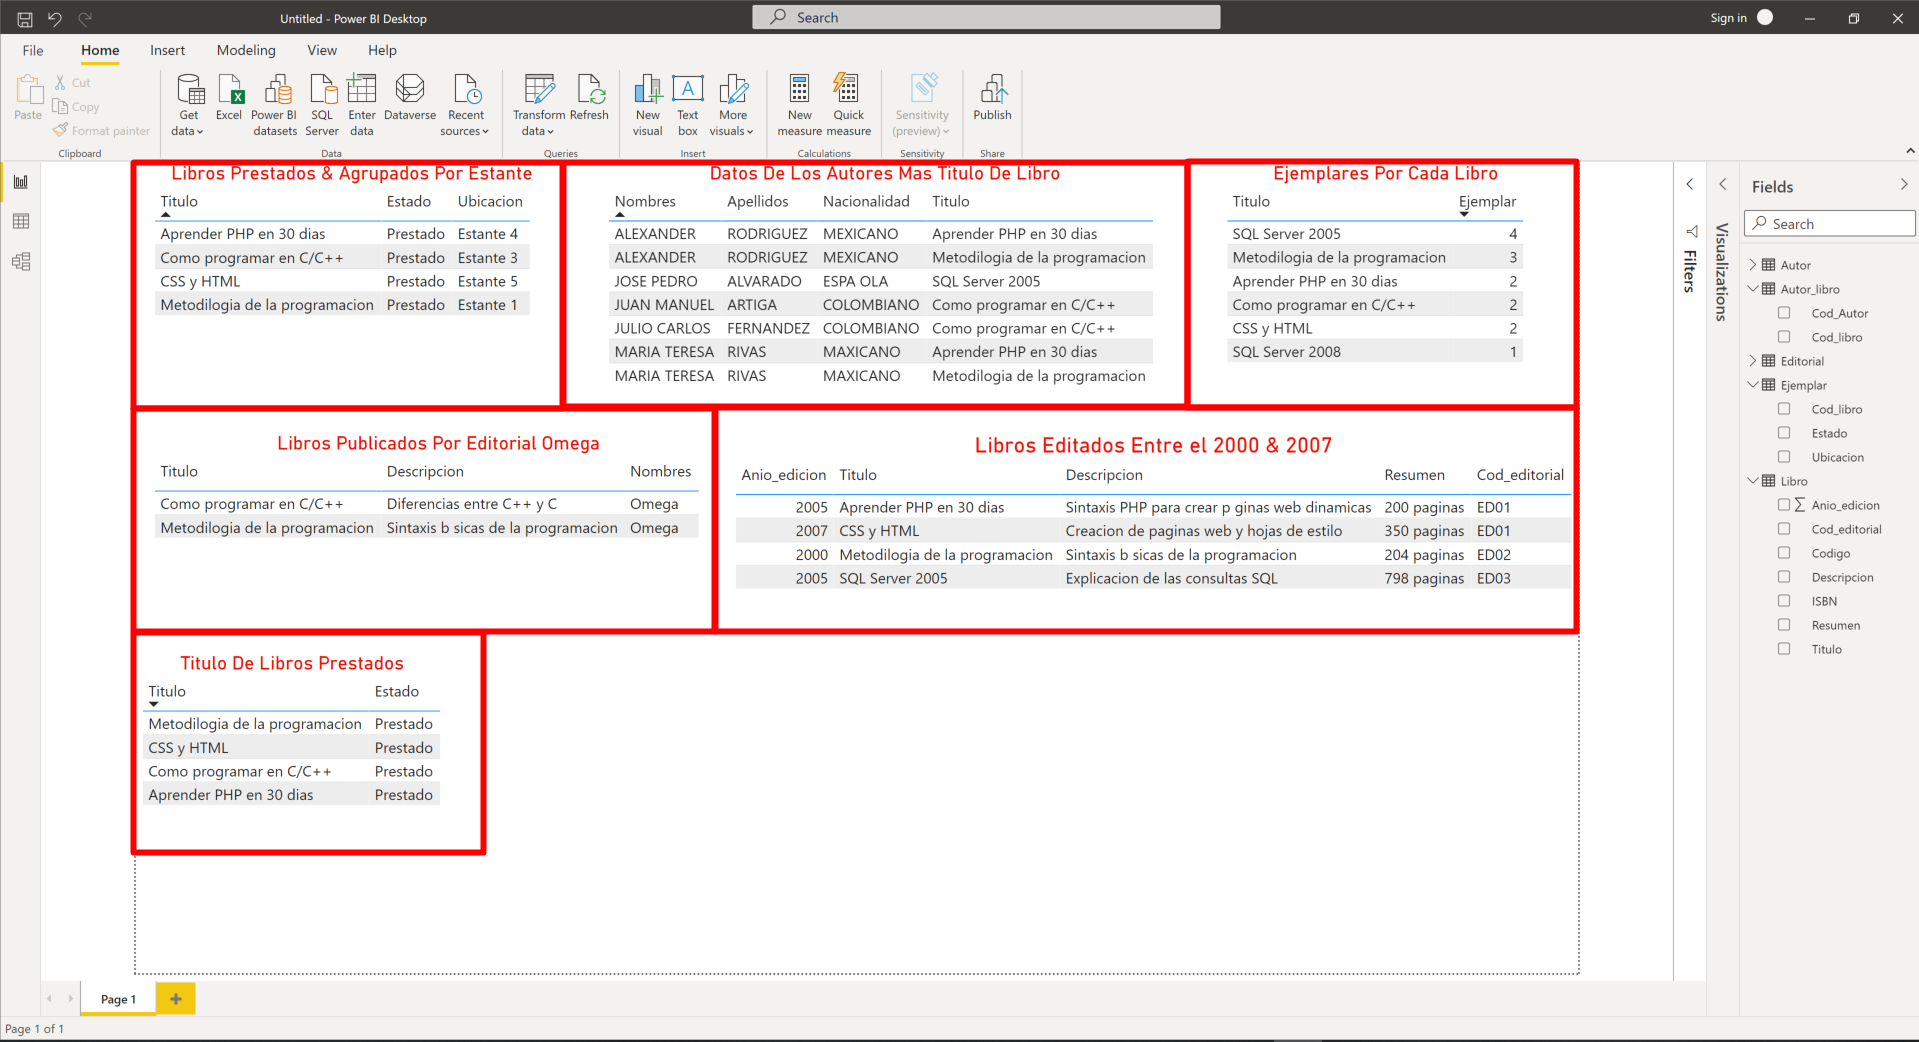
\includegraphics[width=18cm]{img/31.png}  
\end{center}




\end{document}

